\graphicspath{{figures_and_references/EELISA_conference/}}

\renewcommand{\chapternametext}{Chapter \thechapter: Structural system machine learning classifier}

\begin{refsection}

\chapter{\chapternametext}

\renewcommand{\headingtextL}{}
\renewcommand{\headingtextR}{\chapternametext}
\begingroup
\flushbottom
\setlength{\parskip}{0pt plus 1fil}%
\localtableofcontents
\endgroup

\begingroup
\flushbottom
\setlength{\parskip}{0pt plus 1fil}%
\locallistoffigures
\endgroup

\newpage
\setcounter{section}{0}

\renewcommand{\sectionnametext}{Introduction}
\renewcommand{\headingtextL}{\chapternametext}
\renewcommand{\headingtextR}{\thesection. \sectionnametext}
\section{\sectionnametext}
The structural system of a building is a fundamental attribute for seismic risk assessment, yet it is not directly observable through remote sensing or automated footprint extraction. Unlike physical geometric features (such as height, roof, shape, or direction) that can be derived directly from imagery, the structural system depends on internal material properties and load-resisting mechanisms that are not explicitly captured in satellite data.

However, structural typologies are often correlated with observable surrogate attributes, such as building location, the era of construction (represented by the applicable building code), roof material, and footprint irregularity indices. Given the complex, non-linear relationship between these physical/geospatial descriptors and the hidden structural typology, this chapter proposes a machine learning classification workflow. The goal is to statistically infer the most probable structural system, Masonry, Concrete, or Adobe, by learning the underlying patterns identified during the field surveys conducted in our pilot regions.

\section{Dataset}
A classifier is trained using a dataset composed of building samples from three pilot regions: San José, Guatemala City, and Santo Domingo. The dataset is randomly partitioned, allocating 80\% of the instances for training and 20\% for testing. Structural system representation is inherently imbalanced across the regions; in San José, masonry and concrete buildings dominate, while in Guatemala City, adobe and masonry constructions are more prevalent. In Santo Domingo, the majority of structures correspond to high-rise concrete buildings. By combining data from all three regions, a more balanced representation of structural types is achieved, partially mitigating regional biases.

For the classification task, only three structural systems are considered: masonry [M], concrete [CR], and adobe [M99-ADO], as there is insufficient data available for other categories (fig. \ref{fig:structural_system_hist}).

\begin{figure}[htbp]
\centering
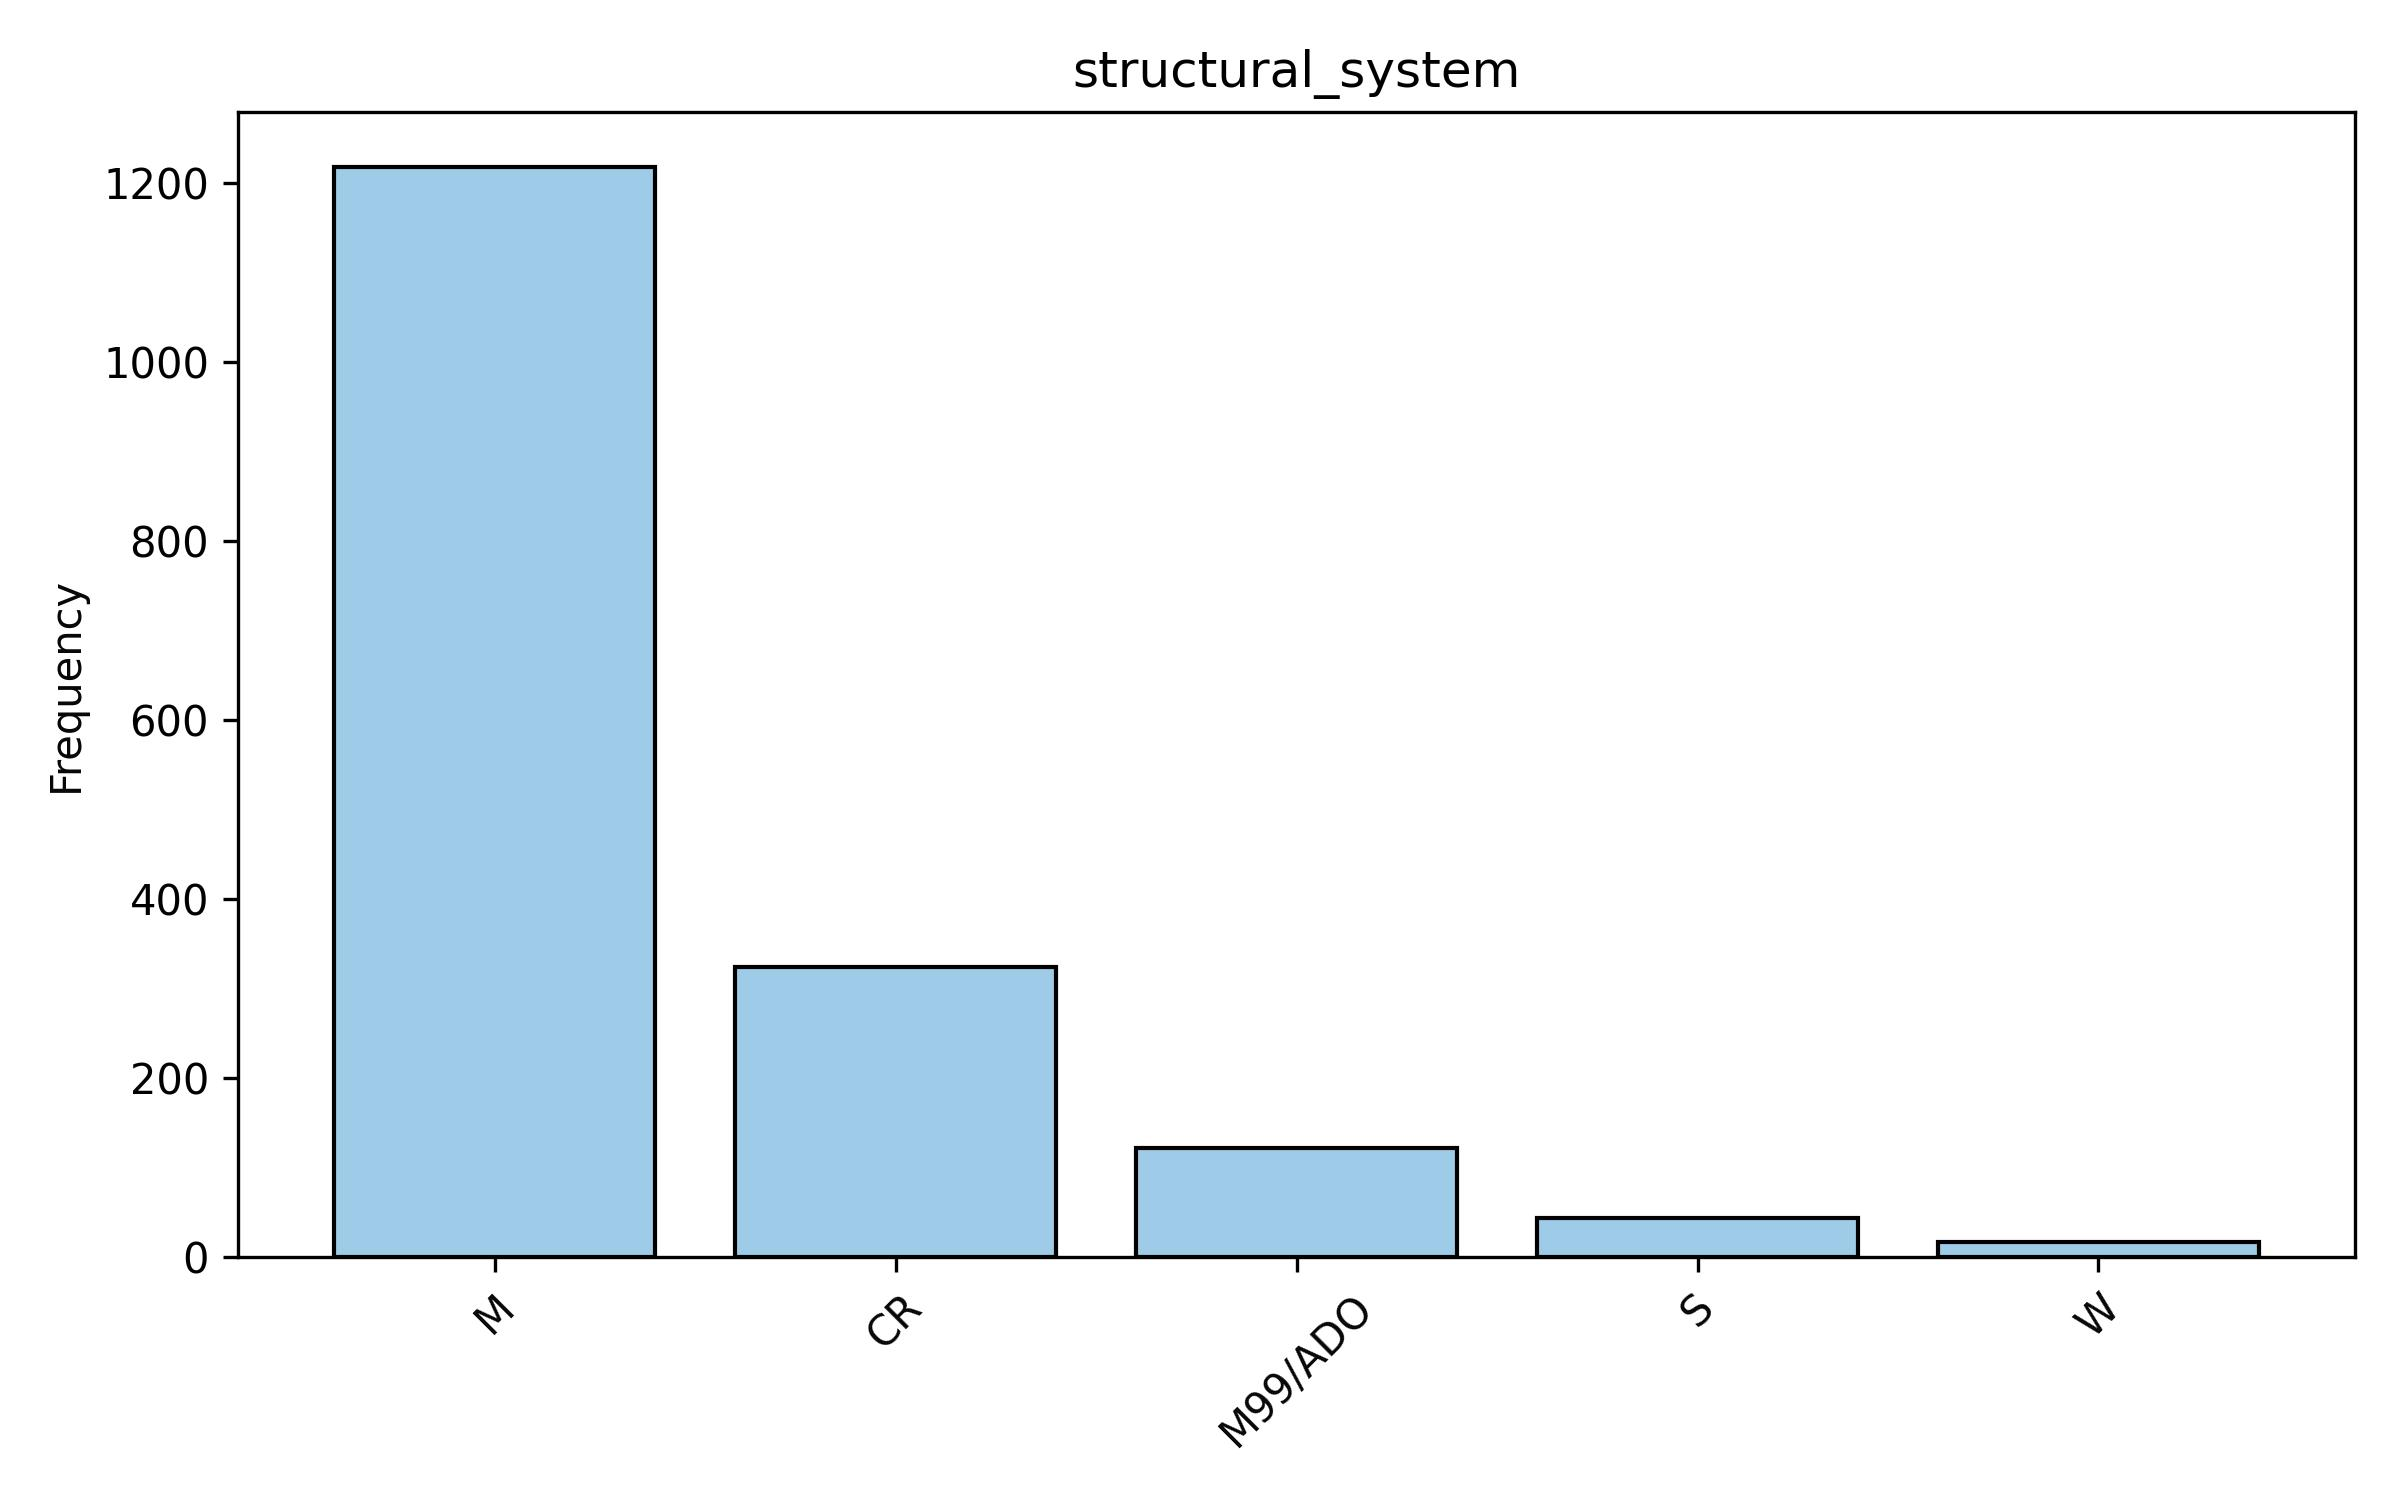
\includegraphics[width=0.5\linewidth]{figures/histogram_structural_system.jpg}
\caption{Histogram of the structural systems in the training dataset.}
\label{fig:structural_system_hist}
\end{figure}

To address residual class imbalance, two conceptual strategies are implemented: the use of class-dependent weighting during model optimization and the application of the synthetic minority oversampling technique (SMOTE) to generate synthetic samples of underrepresented classes.

\section{Models}
We evaluate several algorithmic approaches to determine the most effective classification strategy:
\begin{itemize}
\item \textbf{Multinomial Logistic Regression (LR):} Acts as our baseline model \footcite{bishop_pattern_2016}. It estimates the probability of a building belonging to a class using a linear combination of input features. Its simplicity provides high interpretability regarding the weights of specific geometric and urban features.
\item \textbf{XGBoost:} A gradient-boosted decision tree algorithm \footcite{Chen:2016btl}. It is highly effective at capturing complex, non-linear interactions between features and remains one of the state-of-the-art tools for tabular data classification.
\item \textbf{Random Forest (RF):} An ensemble method consisting of a multitude of decision trees \footcite{parmar_review_2019}. It reduces overfitting through bagging, providing a robust measure of feature importance across the entire dataset.
\item \textbf{TabPFN:} A pre-trained transformer-based foundation model designed for small-to-medium tabular datasets \footcite{hollmann_accurate_2025, hollmann_tabpfn_2023}. Unlike the other models, it is pre-trained to perform "in-context learning," allowing it to achieve high accuracy without extensive hyperparameter optimization cycles.
\end{itemize}

\section{Evaluation}
The experimental procedure follows a rigorous validation pipeline:
\begin{enumerate}
\item \textbf{Feature Preprocessing:} Input features (e.g., eccentricity, compactness, and code-period index) are normalized to ensure all models interpret variables on comparable scales.
\item \textbf{Training and Optimization:} Models are trained on the 80\% subset. For tree-based algorithms, we compare the efficacy of SMOTE against class-weighted loss functions to determine the optimal strategy for the minority (adobe) class.
\item \textbf{Cross-Validation:} We utilize stratified 5-fold cross-validation to assess the stability of model performance across different subsets of data.
\item \textbf{Performance Metrics:} Models are evaluated using weighted F1-scores. This metric is essential for our imbalanced dataset, as it ensures that the performance of the minority classes is not obscured by the overall accuracy of the majority classes.
\end{enumerate}

\newpage
\renewcommand{\sectionnametext}{References}
\renewcommand{\headingtextR}{\thesection. \sectionnametext}
\section{\sectionnametext}
\printbibliography[heading=none]
\end{refsection}